\newpage
\section{Tuning Distance-dependency}\label{sec:tuned_networks}

The discussion in the last section focused on the effect of anisotropy
in connectivity on the occurrence of neuron pair motifs. Could
distance-dependency itself, as imposed by the specific geometry, be a
decisive factor in the distribution of edge counts in neuron pairs?
\textcite{Song2005}, as well as \textcite{Perin2011}, report an
overrepresentation of reciprocal connections independent from
distance-dependent connectivity, opposing the observations made in the
last section (\autoref{fig:two_neuron_probs} A). Furthermore, the
connectivity profile in the anisotropic graph model, as identified in
Section~\ref{sec:distance_connectivity}, follows purely from abstract
geometry rather than being motivated by connectivity found in cortical
circuits. In an attempt to rectify this and to allow for a more
differentiated examination of two neuron connections, in this section
we step away from simplistic geometry and \enquote{tune} the
anisotropic networks to display a distance-dependent connectivity as
reported by Perin et al. by adjusting the width $w(x)$ at any point
$x$ along the axon's projection.

For this we introduce anisotropic networks tuned to reflect a given
distance-dependent connection profile $C(x)$. We are facing the
following problem: Given $C(x):[0,\sqrt{2}) \to [0,1]$, find
$w:[0,\sqrt{2}) \to [0,\infty)$ such that the probability to have a
connection from $v_1$ to $v_2$ for arbitrary vertices $v_1 \neq v_2$
in an anisotropic graph $G(n,w)$ with distance $\mathrm{d}(v_1,v_2) =
x$ is $C(x)$. The problem is in general highly complex when nothing
can be assumed about $C(x)$. We find an approximate solution to the
problem considering the following geometric relation:

\begin{figure}[htp]
  \centering
  \makebox{%
    \begin{overpic}[height=3.35cm]{%
        plots/bed7650b.pdf}
    \end{overpic}
  }%
  \caption{Computing connection probability $C(x)$ from non-constant
    $w(x)$}
  \label{fig:dpp_wc}
\end{figure}

From \autoref{fig:dpp_wc} we have the relation  
\begin{equation}
C\left(\sqrt{x^2+w^2(x)}\right) = \frac{1}{\pi} \operatorname{arctan}
\frac{w(x)}{x}. \label{eq:geo_rel}
\end{equation} 
In order to solve for $w(x)$ we first consider a linear approximation,
expanding
\[C\left(\sqrt{x^2+w^2(x)}\right) \approx C(x) + \left(\sqrt{x^2+w^2(x)} -
x\right) C'(x).\]

The resulting transcendental equation
\[C(x) + \left(\sqrt{x^2+w^2(x)} -
x\right) C'(x) = \frac{1}{\pi} \operatorname{arctan}
\frac{w(x)}{x}\]
is however still too complex in the context of this work. Instead we
propose the approximation $\sqrt{x^2 + w^2(x)} \approx  x$, which
inserting into \ref{eq:geo_rel} yiels
\begin{equation}
C(x) \approx \frac{1}{\pi} \operatorname{arctan} \label{eq:tanapprox}
\frac{w(x)}{x}.
\end{equation}

Under the assumption that $C(x)<\frac{1}{2}$ for all $x$ we obtain the
identity
\begin{equation}
  w(x) = x \tan\left( \pi\, C(x) \right), \label{eq:xtan}
\end{equation} 
being aware that it only holds as well as
approximation~\ref{eq:tanapprox} does. 

Here we use relation~\ref{eq:xtan} to generate anisotropic networks
reflecting the dis\-tance-de\-pendent connectivity profile as found by
\textcite{Perin2011}. For this we finally need to adjust the before
arbitrarily determined side length of the network's surface. Perin et
al.~mapped connectivity in layer 5 of the rat's somatosensory cortex
up to a distance of $\SI{300}{\micro\meter}$. Using this reported
distance connectivity to generate anisotropic networks via
\ref{eq:xtan}, the chosen side length $s$ determines the networks
overall connectivity (\autoref{fig:determine_side_length} A). We
determine $s = \SI{296}{\micro\meter}$ to match the overall connection
probability of $p = 0.116$ as used before and reported by Song et
al.~(\autoref{fig:determine_side_length} B). The obtained value for
$s$ is consistent with the slice thickness of \SI{300}{\micro\meter}
used in Perin et al.'s experiment.


\begin{figure}[htp]
  \centering
  \makebox{%
    \begin{overpic}[height=4.05cm]{%
        plots/6154302f.pdf}
      \put(85.5,57.0){\small\textbf{A}}
      %\put(12,5){\small\textbf{A}}
    \end{overpic}
    \hfill
    \begin{overpic}[height=3.955cm]{%
        plots/ef0e785d.pdf}
      \put(88.5,58.2){\small\textbf{B}}
    \end{overpic}
  }%
  \captionsetup{skip=7pt}
  \caption{\textbf{Network side length adjusted to match overall
      connection probability} Side length of the network's surface
    determines the overall connection probability in the network when
    axon width function $w(x)$ is fixed. \textbf{A)} Connection
    probability declines with rising side length \textbf{B)}
    Determining side length as $s=\SI{296}{\micro\meter}$ to match $p
    = 0.116$ as reported by \textcite{Song2005}. (\smtcite{6154302f},
    \smtcite{ef0e785d})}
  \label{fig:determine_side_length}
\end{figure}



Having determined the neotwork's side length $s$, we're extending the
quiver of generated sample networks for the numerical analysis once
more by the \enquote{tuned anisotropic graphs}\index{tuned
  anisotropic networks}, in which the axon width $w(x)$ was determined
such that the networks reflect Perin's connectivity profile. Analyzing
the obtained axon width function we note that $x \gg w(x)$ holds for
most $x$, justifying the approximation
\[
  \sqrt{x^2 + w^2(x)} \approx x
\] 
\textit{a posteriori} (\autoref{fig:perin_axwidth}). From the 25
generated networks overall connection probability is extracted as $p =
0.1160 \pm 0.0006$ (SEM), as expected from the choice of $s$
(\smtcite{f11dca65}).



% This approximation holds well as long as $x \gg w(x)$. Using the
% relation to tune the axon width to produce anisotropic networks with a
% distance-dependency as reported by Perin et al., we find that for all $x$ is
% strictly greater than $w(x)$  %(\autoref{fig:perin_axwidh


\begin{figure}[htp]
  \centering
  \hspace{0.05cm}
  \begin{overpic}[width=0.6\textwidth]{%
      plots/d45c02e4.pdf}
          \put(69.4,51.5){\small\textbf{A}}
  \end{overpic}
  \hfill
  \begin{overpic}[width=0.35\textwidth]{%
      plots/8f0d65e4.pdf}
    \put(81,86){%
      \fboxsep=2pt\colorbox{white}{\small\textbf{B}}
    }
  \end{overpic}
  \captionsetup{skip=7pt}
  \caption{\textbf{Anisotropic network model with tuned axon width
      $\mathbf{w(x)}$} \textbf{A)} Resulting axon width function
    $w(x)$ from tuning to distance-dependent connection profile as
    reported by \textcite{Perin2011}, see also
    \autoref{fig:perin_profiles}. Note that $x \gg w(x)$ for most $x$,
    supporting approximation~\ref{eq:tanapprox}. \textbf{B)}
    Showing for a single neuron (star) connected (red) and unconnected
    (gray) neurons in the tuned anisotropic network, revealing
    the characteristic axon shape. (\smtcite{d45c02e4}, \smtcite{8f0d65e4})}
  \label{fig:perin_axwidth}
\end{figure}




Overall distance-dependent connection probabilities in the tuned
an\-iso\-tro\-pic graphs clearly match the profile of Perin et
al.~(\autoref{fig:perin_profiles} A), presenting strongest the
argument in support of the chosen approximation. Analyzing two neuron
connections \marginpar{revisiting two neuron connections} in the tuned
networks, we affirm the findings of the last section. In their
experiment, Perin et al.~were able to show an overrepresentation of
reciprocal connections at any inter-neuron distance
(\autoref{fig:perin_profiles} B-C). Rather than matching these
profiles, we find that occurrences of one- and bidirectionally
connected pairs in the anisotropic graphs align with probabilities
obtained from the distance-dependent overall connection probability
$p(x)$ under the assumption of independence (cf. Equation~\ref{eq:pairs}),
\begin{equation*}
  \label{eq:pairs}
  \begin{aligned}%
    & \mathbf{P}_{X=1}(x) = 2p(x) \left(1-p(x) \right)    
      && \text{single connection,}\\
    & \mathbf{P}_{X=2}(x) = p(x)^2        
      &&\text{reciprocal connection.}
  \end{aligned}%
\end{equation*}%
\vspace{0.1cm}%
Thus, in comparison with Perin et al.'s findings, we find that
anisotropy in connectivity cannot account for the overrepresentation
in reciprocal connections. While results in
Section~\ref{sec:two_neuron} still indicated such an
overrepresentation due to distance-dependency, examining the
occurrence of two neuron connections at any inter-neuron distance in
anisotropic networks, tuned to a distance-dependent connection profile
matching experimental findings from cortical circuits, imply complete
unrelatedness of anisotropy and two-neuron connection distributions.

\begin{figure}[htp]
  \centering
  \makebox{%
    \begin{overpic}[width=0.5\textwidth]{%
        plots/875505b0_overall.pdf}
      \put(28,19){\small\textbf{A}}
    \end{overpic}
    \hfill
    \begin{overpic}[width=0.5\textwidth]{%
        plots/875505b0_single.pdf}
      \put(28,19){\small\textbf{B}}
    \end{overpic}
  }%
  \vspace{-0.6cm}
  \makebox{%
    \begin{overpic}[width=0.5\textwidth]{%
        plots/875505b0_recip.pdf}
       \put(28,19){\small\textbf{C}}
    \end{overpic}
    \vspace{-1cm}
    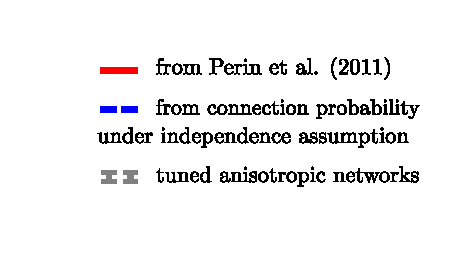
\includegraphics[width=0.5\textwidth]{%
      img/tuned_legend.pdf}   
  }%
  \captionsetup{skip=7pt}
  \caption{\textbf{Distance-independent overrepresentation of
      reciprocal connections} Comparison of occurrences of one- and
    bidirectionally connected neuron pairs in the tuned anisotropic
    networks (gray) with profiles found by Perin et al.~(red), shows
    that overrepresentation of bidirectional pairs is
    distance-independent and not connected to anisotropy.  \textbf{A)}
    Overall connection probability in the tuned anisotropic networks
    was successfully adjusted to reflect connection probability found
    by Perin et al. \textbf{B)-C)} Showing in blue the probabilities
    to obtain a neuron pair motif (single edge in B, two edges in C)
    calculated under independence assumption from the overall
    probability from A), we find that counts in the tuned anisotropic
    networks (gray) match the independence assumption and do
    \textit{not} show the overrepresentation present in Perin et al.'s
    experiment. (\smtcite{875505b0})}
  \label{fig:perin_profiles}
\end{figure}



%%% Local Variables: 
%%% mode: latex
%%% TeX-master: "../dplths_document"
%%% End: 


% \begin{figure}[htp]
%   \centering
%     \begin{minipage}{.45\textwidth}

%         \begin{overpic}[width=\textwidth]{%
%             plots/6154302f.pdf}
%           \put(85.5,57.5){\small\textbf{A}}
%           % \put(12,5){\small\textbf{A}}
%         \end{overpic}
%         \vfill
%         \begin{overpic}[width=\textwidth]{%
%             plots/ef0e785d.pdf}
%           \put(90.5,58.2){\small\textbf{B}}
%         \end{overpic}

%       \end{minipage}
%       \hfill
%       \begin{minipage}{.45\textwidth}

%         \begin{overpic}[width=0.85\textwidth]{%
%             plots/bed7650b.pdf}
%         \end{overpic}
%        \vfill

%         \begin{overpic}[width=0.85\textwidth]{%
%             /users/hoffmann/research/connected_test.pdf}
%           % \put(90.5,58.2){\small\textbf{B}}
%         \end{overpic}
 
        
%       \end{minipage}
      
%   \vspace{-0.15cm}
%   \caption{ (\smtcite{6154302f}, \smtcite{ef0e785d})} %?? fix width issue!!
%   \label{fig:determine_side_length}
% \end{figure}


% \begin{figure}[htp]
%   \centering
%   \makebox{%
%     % \begin{overpic}[height=4.05cm]{%
%     %     plots/6154302f.pdf}
%     %   \put(85.5,57.5){\small\textbf{A}}
%     %   %\put(12,5){\small\textbf{A}}
%     % \end{overpic}
%     % \hfill
%     \begin{overpic}[height=4cm]{%
%         /users/hoffmann/research/connected_test.pdf}
%       % \put(90.5,58.2){\small\textbf{B}}
%     \end{overpic}
%   }%
%   \vspace{-0.15cm}
%   \caption{ (\smtcite{6154302f}, \smtcite{ef0e785d})} %?? fix width issue!!
%   \label{fig:tuned_width}
% \end{figure}